
\newpage
\section{Estimating the CDF and Statistical Functionals}

\textbf{Definition 7.1} The empirical distribution function $\hat{F}_n$ is
the CDF that puts mass 1/n at each data point $X_i$.
$$
\hat{F}_n(x) = \frac{\sum_{i=1}^n I(X_i\leq x)}{n}
$$
where $I(\cdot)$ is the indicator function.

\subsection*{Exercises}

\medskip\noindent
%%%%%%%%%%%%%%%%%%%%%%%%%%%%%%%%%%%%%%%%%%%%%%%%%%%%%%%%%%%%%%%%%%%%%%%%%%%%%%%
\textbf{7.1} - Theorem 7.3\\  % PDF page 104
$$
\E[\hat{F}_n(x)] = F(x)
$$
\textsc{Proof}.
\begin{align*}
    \E[\hat{F}_n(x)] = \E\left[\frac{\sum_{i=1}^n I(X_i\leq x)}{n}\right]
    &= \frac{1}{n} \sum_{i=1}^n \E[I(X_i\leq x)] \\
    &= \frac{1}{n} \sum_{i=1}^n \Big(1\cdot \P(X_i\leq x) + 0\cdot \P(X_i > x)\Big) \\
    &= \frac{1}{n} \sum_{i=1}^n \P(X_i\leq x) = \frac{1}{n}\cdot n\P(X_i\leq x)\\
    &= \P(X_i\leq x) \\
    &= F(x)\tag*{\qed}
\end{align*}
The second identity.
$$
\V(\hat{F}_n(x)) = \frac{F(x)(1 - F(x))}{n}
$$
\textsc{Proof}. Calculating the variance of $I(X_i\leq x)$, starting with the second moment.
$$
\E[I(X_i\leq x)^2] = (1)^2\cdot \P(X_i\leq x) + (0)^2\cdot \P(X_i > x) = \P(X_i\leq x)
$$
The variance.
$$
\V(I(X_i\leq x)) = \E[I(X_i\leq x)^2] - \E[I(X_i\leq x)]^2 = \P(X_i\leq x) - \P(X_i\leq x)^2
= \P(X_i\leq x)(1 - \P(X_i\leq x))
$$
\begin{align*}
    \V(\hat{F}_n(x)) = \V\left[\frac{\sum_{i=1}^n I(X_i\leq x)}{n}\right]
    &= \frac{1}{n^2} \sum_{i=1}^n \V[I(X_i\leq x)] \\
    %&= \frac{1}{n^2} \sum_{i=1}^n \P(X_i\leq x) - \P(X_i\leq x)^2 \\
    &= \frac{1}{n^2} \sum_{i=1}^n \P(X_i\leq x)(1 - \P(X_i\leq x)) \\
    &= \frac{\P(X_i\leq x)(1 - \P(X_i\leq x))}{n} \\
    &= \frac{F(x)(1 - F(x))}{n} \tag*{\qed}
\end{align*}

\newpage\noindent
MSE.
$$
\MSE = \frac{F(x)(1 - F(x))}{n} \ra 0
$$
\textsc{Proof}.
First we need the bias, but as the first result showed, this is an unbiased estimator. 
$$
\bias(\hat{F}_n) = \E[\hat{F}_n] - F_n = F_n - F_n = 0
$$
The MSE is the sum of the squared bias and the variance, but since the bias is 0, it becomes
equal to the variance.
$$
\MSE = \frac{F(x)(1 - F(x))}{n}
$$
As, $n\ra\infty$, this will tend to 0.
\begin{equation*}
    \lim_{n\ra\infty}\MSE = \lim_{n\ra\infty}\frac{F(x)(1 - F(x))}{n} = 0
    \tag*{\qed}
\end{equation*}
The empirical distribution converges in probability to $F(x)$.
$$
\hat{F}_n(x) \raP F(x).
$$
\textsc{Proof}.
Recalling that $\mu = \E[\hat{F}_n] = F_n$ and $\sigma^2 = (F(x)(1-F(x)))/n$. Using Chebyshev's
inequality. For any $\eps > 0$,
$$
\lim_{n\ra\infty}\P(|\hat{F}_n(x) - F_n(x)| > \eps) \leq \lim_{n\ra\infty}\frac{\sigma^2}{\eps^2}
= \lim_{n\ra\infty}\frac{F(x)(1-F(x))}{n\eps^2} = 0.
$$
This shows that $\hat{F}_n(x) \raP F(x)$.\qed

\bigskip\noindent
%%%%%%%%%%%%%%%%%%%%%%%%%%%%%%%%%%%%%%%%%%%%%%%%%%%%%%%%%%%%%%%%%%%%%%%%%%%%%%%
\textbf{7.2}\\  % PDF page 104
For $X_1,\ldots,X_n\sim\text{Bernoulli}(p)$ and 
$Y_1,\ldots,Y_m\sim\text{Bernoulli}(q)$, we will find the plug-in estimator and
estimated standard error for $p$, an approximate 90 percent confidence interval for $p$,
the plug-in estimator and standard error for $p-q$ and approximate 90 percent
confidence interval for $p-q$. (Oh, is that all?)

\medskip\noindent
The plug-in estimator is really just a term for using the $\hat{F}_n$ instead of $F$
for calculating functionals, such as the mean, median etc. For estimating $p$ in
a Bernoulli distribution, it is simply the sample mean.
$$
\hat{p} = \frac{1}{n}\sum_{i=1}^n X_i
$$
Finding the standard error by e.g. using $\hat{p}$ in the variance formula.
$$
\se(\hat{p}) = \frac{\sqrt{\hat{p}(1 - \hat{p})}}{\sqrt{n}}
$$
By consluting a standard normal table we can see that 1.65 is the value that gives 0.95
of the data, which will correspond to a 90\% two-sided test.
$$
\hat{p} \pm z_{.10/2}\se(\hat{p}) = 1.65\cdot\se(\hat{p}) %\imp \hat{p} \pm z_{1.65}\se
$$

\newpage\noindent
Finding an estimate for $p - q$ with a plug-in estimator is simply subtracting the sample means.
$$
\hat{p} - \hat{q} = \frac{1}{n}\sum_{i=1}^n X_i - \frac{1}{m}\sum_{j=1}^m Y_j
$$
The standard error for $\hat{q}$ is:
$$
\se(\hat{q}) = \frac{\sqrt{\hat{q}(1 - \hat{q})}}{\sqrt{m}}
$$
And the combined standard error is:
$$
\se = \sqrt{(\se(\hat{p}))^2 + (\se(\hat{q}))^2},
$$
and in the same way, we can calculate a 90\% confidence interval by using the same
value from the standard normal table.
$$
\hat{p} - \hat{q} \pm 1.65\cdot\se
$$

\bigskip\noindent
%%%%%%%%%%%%%%%%%%%%%%%%%%%%%%%%%%%%%%%%%%%%%%%%%%%%%%%%%%%%%%%%%%%%%%%%%%%%%%%
\textbf{7.3}\\  % PDF page 104
Program code found in \texttt{7.3.R}. There is no technical appendix, so the confidence
intervals are meant to be made with the Dvoretzky-Kiefer-Wolfowitz inequality.

For a 95\% confidence interval, we define
$$
\eps_n = \sqrt{\frac{1}{2n}\log\left(\frac{2}{\alpha}\right)}
$$
where $\alpha = 0.05$ and specify the bounds as
$(\hat{F}_n(x) - \eps_n, \hat{F}_n(x) + \eps_n)$. We simulate 100 $X\sim N(0,1)$ variables
a total of 1000 times and calculate the confidence intervals for each bound, then we count
how many of the 1000 simulations make bounds that do not contain the true CDF.
Illustration of what the simulations look like. (Black is the true CDF, the colored are simulations).
\begin{figure}[H]
    \centering
    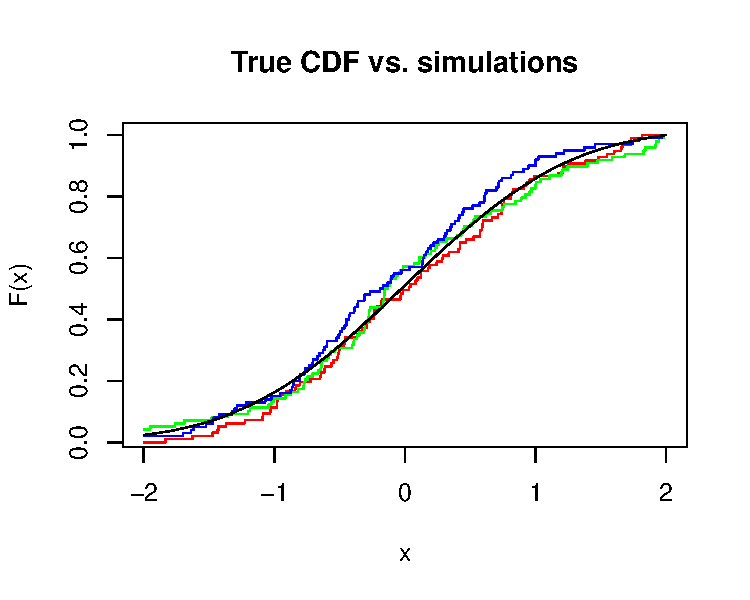
\includegraphics[scale=0.69]{ch7_3.pdf}
\end{figure}

\newpage\noindent
On running the simulation, approximately 95\% of the simulation bounds contained the true CDF.

When redoing for the Cauchy distribution, the results are approximately 95\% as well.
\begin{lstlisting}[style=RSyntax, title=R]
[1] "Proportion of normal distributions containing the CDF"
> sum(checkNorm)/length(checkNorm)
[1] 0.952
[1] "Proportion of Cauchy distributions containing the CDF"
> sum(checkCauchy)/length(checkCauchy)
[1] 0.949
\end{lstlisting}

\bigskip\noindent
%%%%%%%%%%%%%%%%%%%%%%%%%%%%%%%%%%%%%%%%%%%%%%%%%%%%%%%%%%%%%%%%%%%%%%%%%%%%%%%
\textbf{7.4}\\  % PDF page 104
Let $X_1,\ldots, X_n\sim F$ and let $\hat{F}_n(x)$ be the empirical distribution function.
For a fixed $x$, we will use the CLT to find the limiting distribution of $\hat{F}_n(x)$.

\medskip\noindent
We make the definiton:
$$
\bar{Y}_n = \frac{\sum_{i=1}^n I(X_i\leq x)}{n}
$$
to highlight the fact that $\hat{F}_n(x) = \bar{Y}_n$ is a sample mean. By the CLT:
$$
\frac{\sqrt{n}(\bar{Y}_n - \mu)}{\sigma} \raD \mc{N}(0, 1)
$$
where $\mu = \E[\bar{Y}_n]$ and $\sigma^2/n = \V(\bar{Y}_n)$, or the equivalent statement:
$$
\bar{Y}_n \raD \mc{N}(\mu, \sigma^2/n) = \mc{N}(\E[\bar{Y}_n], \V(\bar{Y}_n))
$$
Since $x$ is fixed, we can apply Theorem 7.3:
$$
\E[\bar{Y}_n] = \E[\hat{F}_n(x)] = F(x)
$$
$$
\V(\bar{Y}_n) =\V(\hat{F}_n(x)) = \frac{F(x)[1 - F(x)]}{n}
$$
In summary, when replacing $\hat{F}_n(x)$ for $\bar{Y}_n$, we have shown:
$$
\hat{F}_n(x) \approx \mc{N}\left(F(x), \frac{F(x)[1 - F(x)]}{n}\right)
$$
We can actually apply Chebyshev's inequality in this case. For any $\eps > 0$,
$$
\lim_{n\ra\infty}\P(|\hat{F}_n(x) - F(x)| > \eps) \leq
\lim_{n\ra\infty}\frac{F(x)[1 - F(x)]}{n\eps^2} = 0,
$$
which shows that $\hat{F}_n(x) \raP F(x)$ which again implies $\hat{F}_n(x) \raD F(x)$.

\newpage\noindent
%%%%%%%%%%%%%%%%%%%%%%%%%%%%%%%%%%%%%%%%%%%%%%%%%%%%%%%%%%%%%%%%%%%%%%%%%%%%%%%
\textbf{7.5}\\  % PDF page 104
Let $x$ and $y$ be two distinct points. Find $\Cov\big(\hat{F}_n(x), \hat{F}_n(y)\big)$. 

\medskip\noindent
First of all, introducing the short-hand notation:
$$
I_x := I(X_i\leq x),\qquad I_y := I(X_i\leq y)
$$
Assuming independence of the $X_i$. Then, $\Cov(I_x, I_y) = 0$ whenever $i\not=j$. 
By definition:
\begin{align*}
    \Cov\big(\hat{F}_n(x), \hat{F}_n(y)\big)
    &= \Cov\left(\frac{\sum_{i=1}^n I_x}{n}, \frac{\sum_{j=1}^n I_y}{n}\right) \\
    &= \frac{1}{n^2} \Cov\left(\sum_{i=1}^n I_x, \sum_{j=1}^n I_y \right) \\
    &= \frac{1}{n^2} \sum_{i=1}^n \Cov(I_x, I_y) %\tag{By Ex. 3.14 and ind.}
\end{align*}
The last part follows from the identity proved in exercise 3.14, and from independence, which
leads to all terms with different indices to become 0, hence leaving just a single sum.
Now we will do an intermediary calculation, and we will assume that $x < y$:
\begin{align*}
    \Cov(I_x, I_y) &= \E[I_xI_y] - \E[I_x]\E[I_y] \\
    &= \E[I_x] - \E[I_x]\E[I_y] \tag{Since $x < y$}\\
    &= \E[I_x](1 - \E[I_y]) \\
    &= \P(X_i\leq x)(1 - \P(X_i\leq y)) \\
    &= F(x)\big[1 - F(y)\big] 
\end{align*}
Returning to the main calculation:
\begin{align*}
    \Cov\big(\hat{F}_n(x), \hat{F}_n(y)\big)
    &= \frac{1}{n^2} \sum_{i=1}^n \Cov(I_x, I_y) \\
    &= \frac{1}{n^2} \sum_{i=1}^n F(x)\big[1 - F(y)\big] \\
    &= \frac{1}{n^2}\cdot n\cdot F(x)\big[1 - F(y)\big] \\
    &= \frac{F(x)\big[1 - F(y)\big]}{n}.
\end{align*}
This is provided that $x<y$. But since the covariance is symmetric, then the smallest probability
can always be put in as $x$. Since $F$ is unknown, the plug-in estimator is:
$$
\frac{\hat{F}_n(x)\big[1 - \hat{F}_n(y)\big]}{n}
$$
Note that this is very similar to the expression for the variance.
$$
\V(\hat{F}_n) = \frac{F(x)(1 - F(x))}{n}
$$

\newpage\noindent
%%%%%%%%%%%%%%%%%%%%%%%%%%%%%%%%%%%%%%%%%%%%%%%%%%%%%%%%%%%%%%%%%%%%%%%%%%%%%%%
\textbf{7.6}\\  % PDF page 104
Let $X_1,\ldots, X_n \sim F$ and let $\hat{F}$ be the empirical distribution function.
For $a<b$ define $\theta = T(F) = F(b) - F(a)$ and set
$\thetah = T(\hat{F}_n) = \hat{F}_n(b) - \hat{F}_n(a)$. Find the estimted standard error of $\thetah$
and an expression for the $1-\alpha$ confidence interval for $\theta$.

Following example 7.15, the standard error of a difference is the square root of the following variances:
\begin{align*}
    \se(\thetah) &= \sqrt{\V(\hat{F}_n(b) - \hat{F}_n(a))} \\
    &= \left(\V(\hat{F}_n(b)) + \V(\hat{F}_n(b)) - 2\Cov(\hat{F}_n(a), \hat{F}_n(b))\right)^{\frac{1}{2}} \tag{Prop. of var.}\\
    &= \frac{1}{\sqrt{n}}\left(F(b)[1 - F(b)] + F(a)[1-F(a)] - 2F(a)[1-F(b)]\right)^{\frac{1}{2}} \tag{Thm 7.3, Ex. 7.5} \\
    &= \sqrt{\frac{(F(b) - F(a))[1 - (F(b) - F(a))]}{n}} \tag{See notes.}\\
    &= \sqrt{\frac{(\hat{F}_n(b) - \hat{F}_n(a))[1 - (\hat{F}_n(b) - \hat{F}_n(a))]}{n}} \tag{Plug-in est.}\\
    &= \sqrt{\frac{\thetah(1 - \thetah)}{n}} \tag{Def. of $\thetah$}
\end{align*}
Finding the confidence interval is easy. Just find the corresponding $z_{\alpha/2}$ level and calculate:
$$
\thetah \pm z_{\alpha/2}\se(\thetah).
$$
For the sake of clarity, here are the notes for the algebra steps used in the step above.
Instead of $F(b)$ and $F(a)$ we just write $b$ and $a$.
\begin{align*}
    b(1-b) + a(1-a) - 2a(1-b) &= b - b^2 + a - a^2 - 2a + 2ab \\
    &= b - b^2 - a - a^2 + 2ab \\
    &= b - a - b^2 + 2ab - a^2 \\
    &= b - a - (b^2 - 2ab + a^2) \\
    &= b - a - (b-a)^2 \\
    &= (b - a)\big[1 - (b-a)\big]  
\end{align*}

\newpage\noindent
%%%%%%%%%%%%%%%%%%%%%%%%%%%%%%%%%%%%%%%%%%%%%%%%%%%%%%%%%%%%%%%%%%%%%%%%%%%%%%%
\textbf{7.7}\\  % PDF page 104
Code found in \texttt{7.7.R}. Plot of empirical distribution and bounds:
\begin{figure}[H]
    \centering
    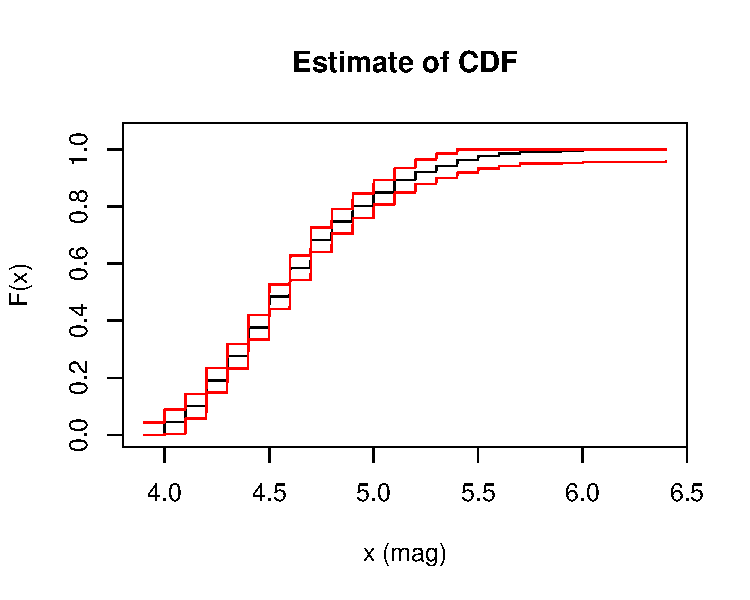
\includegraphics[scale=0.7]{ch7_7.pdf}
\end{figure}
(The CDF jumps because there are only 1000 points and jumps in the data itself).

\medskip\noindent
Finding the confidence interval for $F(4.9) - F(4.3)$. (Note: these results will
differ depending on whether the empirical distribution is defined with $<$ or $\leq$.
These are the bounds for $\leq$, as the definition says).

\begin{lstlisting}[style=RSyntax, title=R]
'95% Confidence Interval for F(4.9) - F(4.3):'
( 0.495 , 0.557 )
\end{lstlisting}

\bigskip\noindent
%%%%%%%%%%%%%%%%%%%%%%%%%%%%%%%%%%%%%%%%%%%%%%%%%%%%%%%%%%%%%%%%%%%%%%%%%%%%%%%
\textbf{7.8}\\  % PDF page 105
Results for the 'Old Faithful' dataset. Code found in \texttt{7.8.R}.

Output from code:
\begin{lstlisting}[style=RSyntax, title=R]
> # Mean
> sprintf("Sample mean: %2.3f", Xbar)
[1] "Sample mean: 70.897"

> # 90% confidence interval
> sprintf("90%% Confidence interval: (%.3f, %.3f)", CIlower, CIupper)
[1] "90% Confidence interval: (48.576, 93.218)"

> # Median
> sprintf("Median at: %2.f, with probability %2.2f", xvalMedian, Fhat(xvalMedian, of$waiting))
[1] "Median at: 76, with probability 0.53"
\end{lstlisting}

\bigskip\noindent
%%%%%%%%%%%%%%%%%%%%%%%%%%%%%%%%%%%%%%%%%%%%%%%%%%%%%%%%%%%%%%%%%%%%%%%%%%%%%%%
\textbf{7.9}\\  % PDF page 105
Comparing two trials of antibiotic. 100 people are given standard and 90 recover,
100 are given new and 85 recover.

\medskip\noindent
We will assume that these are independent. We will also assume that the
standard trial is $X_1,\ldots, X_{100}\sim\text{Bernoulli}(p_1)$ and the new trial is
$Y_1,\ldots, Y_{100}\sim\text{Bernoulli}(p_2)$. This is the same conditions
as in exercise 7.2.

If we define $X_i = 1$ and $Y_i = 1$ for recoveries and $X_i = 0$ and $Y_i = 0$
for no change, we can estimate the probabilities with the sample mean:
$$
\hat{p}_1 = \frac{1}{100}\sum_{i=1}^{100} X_i = \frac{90}{100} = 0.90
$$
$$
\hat{p}_2 = \frac{1}{100}\sum_{i=1}^{100} Y_i = \frac{85}{100} = 0.85
$$
If we define $\thetah = \hat{p}_1  - \hat{p}_2$, it becomes:
$$
\thetah = \hat{p}_1  - \hat{p}_2 = 0.90 - 0.85 = 0.05
$$
Finding the standard errors for each $\hat{p}_i$.
$$
\se(\hat{p}_1) = \frac{\sqrt{\hat{p}_1(1 - \hat{p}_1)}}{\sqrt{n}} = \frac{\sqrt{0.9(0.1)}}{\sqrt{100}} = 0.03
\imp \se(\hat{p}_1)^2 = 0.0009
$$
$$
\se(\hat{p}_2) = \frac{\sqrt{\hat{p}_2(1 - \hat{p}_2)}}{\sqrt{n}} = \frac{\sqrt{0.85(0.15)}}{\sqrt{100}} = 0.0357
\imp \se(\hat{p}_1)^2 = 0.001275
$$
Since they are independent, the covariance is 0. The standard error for $\thetah$:
$$
\se(\thetah) = \sqrt{\V(\hat{p}_1 - \hat{p}_2)} = \sqrt{\se(\hat{p}_1)^2 + \se(\hat{p}_2)^2}
= \sqrt{0.002175} = 0.046637
$$
For constructing the confidence intervals, we find the corresponding $z_{.90}$ and $z_{0.975}$ values
and calculate. Since probabilities can't be negative, we cap them at 0.
80\% confidence interval.
$$
\thetah \pm z_{.90}\se(\thetah)  = 0.05 \pm 1.28(0.046637) = (-0.0097, 0.1097) = (0, 0.1097)
$$
95\% confidence interval.
$$
\thetah \pm z_{.975}\se(\thetah)  = 0.05 \pm 1.96(0.046637) = (-0.0414, 0.1414) = (0, 0.1414)
$$
%%%%%%%%%%%%%%%%%%%%%%%%%%%%%%%%%%%%%%%%%%%%%%%%%%%%%%%%%%%%%%%%%%%%%%%%%%%%%%%
\textbf{7.10}\\  % PDF page 105
Code found in \texttt{7.10.R}.
\begin{lstlisting}[style=RSyntax, title=R]
> theta   # Estimate of theta
[1] 277.3962
> seTheta # Standard error of theta
[1] 388.522
> sprintf("CI: (%3.2f, %3.2f)", CIlwr, CIupr)
[1] "CI: (0.00, 601.90)"
\end{lstlisting}





\begin{comment}

\bigskip\noindent
%%%%%%%%%%%%%%%%%%%%%%%%%%%%%%%%%%%%%%%%%%%%%%%%%%%%%%%%%%%%%%%%%%%%%%%%%%%%%%%
\textbf{7.X}\\  % PDF page 105


\begin{align*}
    A &= B
\end{align*}


\begin{equation*}
    A = B
    \tag*{\qed}
\end{equation*}


\begin{lstlisting}[style=RSyntax, title=R]
# Code
\end{lstlisting}

\begin{verbatim}
# Output
\end{verbatim}





%%%%%%%%%%%%%%%%%%%%%%%%%%%%%%%%%%%%%%%%%%% Figure
\begin{figure}[H]
    \centering
    \includegraphics[scale=0.7]{IMG1.pdf}
\end{figure}



%%%%%%%%%%%%%%%%%%%%%%%%%%%%%%%%%%%%%%%%%%% Minipages x 2
\begin{figure}[H]
    \begin{minipage}{0.5\textwidth}
        % MINIPAGE 1
    \end{minipage}
    \begin{minipage}{0.5\textwidth}
        % MINIPAGE 2
    \end{minipage}
\end{figure}

%%%%%%%%%%%%%%%%%%%%%%%%%%%%%%%%%%%%%%%%%%% Two R images
\begin{figure}[H]
    \begin{minipage}{0.5\textwidth}
    \begin{center}
        \begin{figure}[H]
            \includegraphics[scale=0.7]{IMG1.pdf}
        \end{figure}
    \end{center}
    \end{minipage}
    \begin{minipage}{0.5\textwidth}
    \begin{center}
        \begin{figure}[H]
            \includegraphics[scale=0.7]{IMG2.pdf}
        \end{figure}
    \end{center}
    \end{minipage}
\end{figure}


%%%%%%%%%%%%%%%%%%%%%%%%%%%%%%%%%%%%%%%%%%% Two TikZ images
%%% Tikz Image - side by side
\begin{figure}
    \begin{minipage}[0.5\textwidth]
\begin{tikzpicture}
    \begin{axis}[
        width=\textwidth,
        axis lines = left,
        ymin = -0.002,
        ymax = 2.1,
        xlabel = $z$,
        ylabel = {$f_Z(z)$},
    ]
    %Section 1
    \addplot [
        domain=0:1, 
        samples=10, 
        color=blue,
        style=ultra thick,
    ]
    {2 - 2*x};
    \end{axis}
\end{tikzpicture}
    \end{minipage}
    \begin{minipage}[0.5\textwidth]
\begin{tikzpicture}
    \begin{axis}[
        width=\textwidth,
        axis lines = left,
        ymin = -0.002,
        ymax = 2.1,
        xlabel = $z$,
        ylabel = {$f_Z(z)$},
    ]
    %Section 1
    \addplot [
        domain=0:1, 
        samples=10, 
        color=blue,
        style=ultra thick,
    ]
    {2 - 2*x};
    \end{axis}
\end{tikzpicture}
    \end{minipage}
\end{figure}

    
    
\end{comment}